\chapter{Concept}
\label{sec:concept}

One of the main goals of this work is to describe and implement a framework that allows for quantitive statements about differences between user selected regions of importance and computer generated mesh saliency maps to be made. It also includes such a comparison on a basic, conceptual level. Based on these abstract tasks given, the workload and how it is apporached, can be described by the following milestone-like, high level requirements.

\begin{enumerate}
	\item implement a selection application for an immersive virtual reality environment
	\begin{enumerate}
		\item spatial indexing of 3D data
		\item selection process
	\end{enumerate}
	\item conduct a user study to acquire data for a comparison
	\item conceptualise a measure of differences between the data sets
\end{enumerate}

In this section, I will go through these requirements and describe in more detail what specific challenges they entailed and how I went about implementing solutions to them. I will also describe the underlaying concepts I chose to use and how I amended them to better fit this work where needed.

	\section {Implementing a selection application for an immersive VR environment}
	\label{sec:implementing_selection_application_v2c}
One of the main challenges of this work is developing a piece of software that allows users in an immersive VR environment to select vertices of 3D objects. Designing, implementing and adjusting this software to being executable as a multi-threaded client-server application is another challenging aspect of this work. For the rest of this work, this piece of software will be refferend to as \textit{selection application}. For details on its implementation, see section \ref{sec:selection_application}.

		\subsection{Spatial indexing of 3D data}
		\label{sec:impl_spatial_indexing_3d}
3D objects and data in general are read as lists of coordinates by computers. Common 3D file formats such as .OBJ, .FBX and .STL contain the same data in similar structures, using multiple lists of different kinds of geometric information. While they these formats vary in the range of information they can hold, they all represent at least the following types of essential data. \textit{Vertices}, or a three tuple of float values describing x, y and zu coordinates and \textit{faces}, or basic triangles consisting of three vertices. Other optinal information that can be represented include vertex normals, texture coordinates and more complex features such as assigned materials, animations and armature objects. Figure \ref{fig:obj_content} shows an excerpt of a 3D file in .OBJ format, viewed in a simple text editor (gedit).

\begin{figure}[htb]
  \centering
  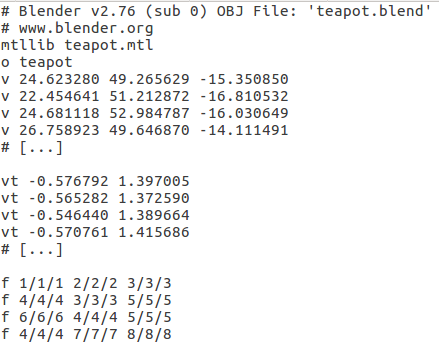
\includegraphics[width=.6\textwidth]{obj_content.png}\\ % PNG-File
  \caption{Notation in .OBJ format}\label{fig:obj_content}
\end{figure}

All these types of information share the following properties which were of relevance for this work. They are contiguous lists of lines, each line representing one instance of the data type indicated in the beginning of the line. Figure \ref{fig:obj_content} depicts an excerpt of an .OBJ file ocntaining vertices (lines starting with v), vertex texture coordinates (lines starting wit vt) and faces (lines starting with f).

These lists are not ordered. Depending on the modelling process, the vertices, faces and all the other attributes can be presented in an completely arbitrary order which hold very little information about the actual, geometric features of the object. The spatial position of any given vertex in relation to the entire object can not be retrieved from this type of notation. This created the demand for spatially indexing of 3D data in the scope this work.

I decided to implement the concept of Octrees \cite{Octree} because of its convenient characteristics as well as prior, personal working experience with \textit{quadtrees}. In an octree, the geometric size of the smallest possible leaf node can be determined in direct relation to the object to be indexed and, at any level, all leafs and nodes will be of the same size. This is highly useful in radius-based proximity-requests for multipl reasons as described in section \ref{sec:addVerticesToSelectionByCoordinates()}.

\begin{figure}[htb]
  \centering
  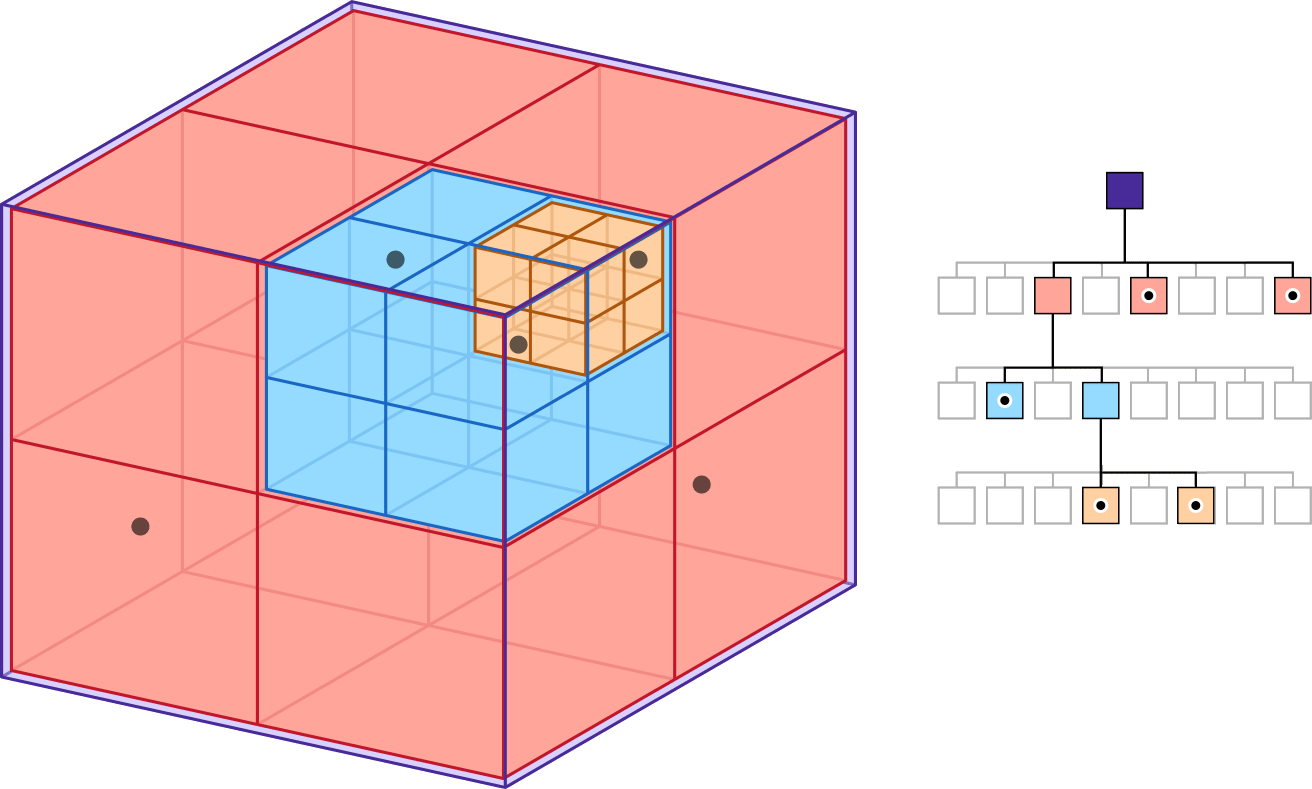
\includegraphics[width=.9\textwidth]{ocTree_appleb.png}\\ % PNG-File
  \caption{An octree structure indexing five vertices. Left: 3D view, right: tree structure; 2017, https://developer.apple.com/documentation/}\label{fig:ocTree_apple}
\end{figure}

One of the most common queries performed on 3D data are proximity queries. This means that vertices located within a given radius around an input query-coordinate are to be retrieved. The trivial and obviously highly inefficient solution to such a problem would be to iterate through the entire list of vertices and their coordinates and check for those who fulfill this query condition. This is where spatial indexing structures such ad octree come into play. The concept of octrees is highly recursive and can realize all the most common types of queries (including search queries) in logarithmic time.

An octree is a set of nodes that store references to one another. The highest-level node is called the root node, bottom level nodes are usually referred to as leaf nodes or leafs. Every node that is not a leaf node has eight children-nodes which, in a spatial sense, make up the entire space of their parent node. Such non-leaf nodes can also be described as roots of subtrees.

Figure \ref{fig:ocTree_apple} taken from \cite{octAp} shows a simple octree structure indexing five vertices, both in 3D and tree view. Note how the root node on level 0, shaded purple on the right, is represented as a large purple cube on the left, encompassing the entire set of vertices. The figure visualizes how an non-balanced octree structure that allows one vertex per leaf node at most would look like. On levels 1, 2 and 3, there are eight nodes each. On level 1 (shaded red), there are two leaf nodes that hold one vertex each. The eighth subtree node contains three vertices and is thus split into eight subtree nodes (shaded blue), each on level 2. Out of these level 2 subtree nodes, one is split again into eight level 3 leaf nodes, two of which store one vertex each.

The most important parameter for an octree is the maximum allowed number of vertices per leaf node. Once the dimensions in x-,y - and z-direction of the 3D object to be indexed have been determined, the root node of the octree will store every vertex until said maximum allowed number of vertices is reached. Up until that point, the root node is a leaf. It is from then on no longer a root and creates eight new nodes (its child nodes) and store references to them. This process is repeated recursively for every new node until every leaf node holds less than the maximum allowed number of vertices per leaf node. It is worth mentioning that in many implementations of the octree concept, every leaf node needs to be at the same level. For this work, the non-balanced version of an octree where that is not the case is used. The reason for this is that in 3D objects, the data is not evenly and very sparsely distributed inside the entire space defined by its bounding box that. The vertices make up the surface of the model, inside and outside of it, there is no spatial information to be indexed at all. Queries to an octree structure can be processed with logarithmic costs which, in combination with sparsely distributed data, allows for fluent, real-time interaction with objects up until a certain magnitude of vertices total. By carefully choosing suitable values for the maximum allowed number of vertices per leaf node and maximum allowed split depth, acces times can be further optimsed.

		\subsection{Selection process}
		\label{sec:selection_process}

To gather data to compare with computer generated mesh saliency maps, tracking user input is needed. In an appropriate immersive virtual reality setup, 3D objects get loaded and spatially indexed using octrees as described in the section above. Now, the selection function is comes into play. Using a handheld input device, users can interact with the scene in two essential ways - navigation and performing arbitrary operations mapped to the device's buttons. Each such operation can, among other information, use the current position and rotation of the wand as parameters. Figure \ref{fig:concept_hardware} in section \ref{sec:hardware_used} shows an example of such an input device.



Figure \ref{fig:wand} depicts the \textit{wand} used in the V2C. The yellow joystick in the middle of its top side, in combination with the current rotation of the device, can be used to navigate the user's view onto the scene. Furthermore, the two essential functions of the application, selecting and deselecting vertices, are mapped to two buttons of the device. From a user perspective, both these functions are executed in a radius around the tracked position of the device. Put simply, vertices that are rendered near the device at the time the user presses buttons, become either part of the current selection or get removed from it. In accordance with the simplistic structure of the user study, the interaction is designed to be as little complex as possible, hence only these two buttons having actual, distinct purposes. 

With this setup in place, everything needed to implement the user selection part of the application is at hand. In order to provide as much visual accuracy as possible, a bright green diamond shaped object at the tracked position of the \textit{wand} is projected into the scene in addition to the loaded model. To additionally provide clear visual feedback, vertices selected are painted in bright red, clearly seperating them from non-selected parts of the object, displayed in plain grey. For more details on the visual presentation of the application, see section \ref{sec:conduct_user_study_with_the_selection_application}.

Whenever a user presses the button the \textit{add} function is mapped to, a proximity query is performed on the octree structure indexing the object with its current position as the input. The position is passed as a three-dimensional coordiante. For a detailed description of how such a query is handled in this application, see section \ref{sec:addVerticesToSelectionByCoordinates()}.

In addition to these input coordinates, the following two parameters are passed to calls to this function in the context of a user adding or removing vertices to the current selection: The pre-computed selection radius and a reference to a temporary set vertices, holding unique vertex IDs. After a query is terminated, the set of vertices found will be added to this temporary set. Due to the design of the synchronisation routine between server and client threads of this application, this set will be emptied before the result of each such query is returend and written to it. If the \textit{add} button is pressed, the content of the intermdiate selection will be added to another set holding the list of currently selected vertices total. If the \textit{remove} button is pressed, each of the temporarily selected vertices is looked up in this second set and, in case it is found, removed from it. This approach prevents the total set of selected vertices to be sent from the server to all client threads at every frame during runtime. Only newly selected vertices (or those that are to be removed from the current selection) are sent across the application. The time for each action (in seconds since the application was started) is logged as well. For more details on the implementation of the \textit{selection application}, see chapter \ref{sec:selection_application}.

	\section {Conduct user study with the selection application}
	\label{sec:conduct_user_study_with_the_selection_application}
Another essential part of this work is conducting a user study where all of the aspects described in this chapter so far are be put to use. The goal is to collect data on what parts of 3D objects users find visually interesting or important. Users put on the stereoscopic, trackable glasses, step inside a suitable immersive VR environment, for example a multi-sided projection installation, and are asked to mark regions of the object currently displayed that they consider to be intersting or important.

After taking a few minutes to get familiar with navigating and interaction within the projection installation, as well as selecting and deselecting vertices with the handheld input device, the main part of the user study begins. For a detailed documentation of how the user study was designed and executed, see chapter \ref{sec:user_study_chapter}.

Selections of the users are gathered to compute user-weighted importance maps for the displayed 3D objects. These are compared to previously computed mesh saliency maps. For the rest of this work, they will be referred to as \textit{user saliency} values. For the results and discussion of this comparison, see chapter 
% @TODO ref zu chapter "results usw" 1fügen. Selbiges davor noch anlegen

In this selection application, selection and deselection operations are executed with the current tracked position of the handheld device as input coordinates. To give users a clear, live feedback on that tracked position, for every frame, a ten-sided, diamond-shaped object is also rendered in the scene on that very position. The object is shaded in a bright green, to be easily distinguishable within the 3D scene. However, it did not offer a visual representation of the pre-computed selection radius. This radius $r_{max}$ is defined as $d_{min}$ / $2^{l_{max}}$ * 0.95, in other words 95\% the size of the smallest possible leaf node, so it is slightly different for every object loaded in the application. The size of the ten-sided object representing the tracked position of the device within the scene is chosen to stay the same for each object and not to adapt to their sizes. This is done with the intention of providing more consistency within the scene, independent of the currently loaded object. This design decision goes in accordance with the minimalistic general visual presentation of the application, as described in the following brief summary.

\begin{itemize}
	\item background-color of the application: (almost) black
	\item shader used for the loaded object: light grey, no textures, normals used
	\item shader used for selected vertices: bright red
	\item shader used for diamond-shaped object indicating the tracked position of the \textit{wand}: bright green
\end{itemize}

Two steps are taken to eliminate the possibility of user selections being influenced by them first having to adapt to and getting familiar with the selection application. First, Every user is given as much time as desired to get familiar with the navigation and selection workflow, accompanied by hints and instructions. Selections made here are not considered for the results of the userstudy. After that - when the user feels ready - the three objects are presented in a randomly chosen order for five minutes each. The users are given the tasks stated at the beginning of this section and are free to use as much of the five minutes as they want to perform vertex selection and deselection operations.

The five minute time limit is an absolute upper limit for each selection process. Users are free to end selection prematurely whenever they state they are satisfied with the selection as it is. See figure \ref{fig:selection_cave} in section \ref{sec:hardware_used} for a basic depiction of what the the interaction looks like in the five-sided projection installation used for this work.

Besides the five minute \textit{tutorial phase} - the time users can take to get familiar with the application - and the actual tasks to be fulfilled (as described at the beginning of this section), a few more instructions are given and requests asked for. Users are asked to consider symmetry in their selection, meaning that, in cases where it is possible, parts of objects users select on one side of the object are also selected on the opposite side. Users are told that there is no \textit{correct} way to fulfill the selection task. They are encouraged to select whatever tehy deem relevant according to the tasks based on their personal judgement and subjective interpretation of \textit{interesting}. The users are left alone during the selection process. After four of the maximum five minutes have passed, users are told that they have one minute remaining. After five minutes, the current selection process is stopped, the result written to a logfile and the next object gets loaded into the VR environment. 


	\section {Measure of differences}
	\label{sec:measure_of_difference}
Since large portions of the workload of this work is the implementation of the selection application as well as conducting the user study, the comparison of user generated and pre-computed mesh saliency maps is designed to be quick and easy. The main goal is to have a ratio that expresses whether there are major differences to be further examined or not.

This chapter describes a basic way to compute a \textit{difference ratio}, normalised to a decimal value between 0 and 1, describing how much user saliency maps differ from mesh saliency maps, is conceptualised. It is based on a simple vertex-wise comparison of saliency-values and makes use of the proximity queries provided by the octree structure, which is also the basis for the selection application itself as described in section \ref{sec:spatial_indexing_via_octree}.

In chapter % @TODO ref zu chapter "results usw" 1fügen. Selbiges davor noch anlegen
I consider both \textit{raw} and \textit{weighted difference} values, for a detailed explanation of these terms, see the following subsections. For a brief summery and step-wise explanation, see subsection \ref{sec:ste_wise_summery}.

		\subsection{Terms and abbreviations}
		\label{sec:concept_terms_and_abbreviations}
The following terms, symbols and abbreviations will be used in the subsequent sections to explain the measure of difference used in this work.

\begin{description}
	\item[unweighted difference ratio] - a float number, normalised to a value between 0.0 and 1.0 indicating how much the generated \textit{user saliency map} differs from the pre-computed \textit{mesh saliency map}, based on unweighted (raw) difference values
	\item[weighted difference ratio] - a float number, normalised to a value between 0.0 and 1.0 indicating how much the generated \textit{user saliency map} differs from the pre-computed \textit{mesh saliency map}, based on weighted difference values
	\item[$v_i$] - the currently considered vertex \textit{i} $\in$ set of all vertices $V$ belonging to an object
	\item[$S_{M}(v_i)$] - the computed mesh saliency value for $v_i$ as described in \cite{lee2005mesh}
	\item[$S_{U}(v_i)$] - the user generated saliency value for $v_i$, describing its \textit{perceived importance} value based on how many users selected it in relation to the most-selected vertices.
	\item[$\Delta_{raw}(v_i)$] - the unweighted (raw) difference between the user and mesh saliency values $S_{U}(v_i)$ - $S_{M}(vi_i)$. The absolute value of the result is normalised to a value between 0.0 and 1.0
	\item[$\Delta_{weighted}(v_i)$] - the weighted difference between the user and mesh saliency values $S_{U}(v_i)$ - $S_{M}(vi_i)$. The absolute value of the result is normalised to a value between 0.0 and 1.0
	\item[$V_{proximty}(v_i)$] - a \textit{proximity set} of vertices $v_1$, ... $v_j$ that are located within radius $r$ around the coordinates of given vertex $v_i$
	\item[$\omega$] - a threshold value for \textit{mesh saliency} values $S_{M}(v_1)$, ... $S_{M}(v_j)$ for all vertices $v_1$, ... $v_j$ $\in$ a \textit{proximity set} $V_{proximty}(v_i)$ of $vi$. $0.8$ is used in this work.
\end{description}

		\subsection{unweighted difference ratio}
		\label{sec:unweighted_difference_ratio}
As stated above, $\Delta_{raw}(v_i)$, or the unweighted (raw) difference between user generated and computed mesh saliency value can easily be obtained by taking the absolute value of $S_{M}(v_i) - S_{U}(v_i)$. For each of the objects used in the user study a mesh saliency map using \texttt{climberpi's} implementation of \textit{mesh saliency} \cite{clms} is computed, providing $S_{M}(v_i)$ for every vertex $v$ in $V_{bunny}$, $V_{cow}$ and $V_{P-51}$ where $V_{l}$ is the set of all vertices that make up the object with label $l$.

Values $S_{U}(v_i)$ are computed via a simple, average-based comparison of how many users selected each vertex. As mentioned in \ref{sec:user_selection}, user selections are written to simple structured text files containing one unique vertex ID and the time they are added to or removed from the selection (in seconds since the application was started) in every line, seperated by a tab symbol as depicted in table \ref{tab:user_selection_log_file}.

\begin{table}[]
\centering
	\begin{tabular}{l|l}
	vertId & timestamp \\ \hline
	27 & 64 \\
	59 & 62 \\
	63 & 62 \\
	64 & 62 \\
	65 & 62 \\
	67 & 62 \\
	68 & 62 \\
	69 & 62
	\end{tabular}
	\caption{Sample content of a user selection log file}
	\label{tab:user_selection_log_file}
\end{table}
% table 3.3

In the simple evaluation process used for this work, before each logfile is read, a container object \textit{user selections} is created with size equivalent to the number of vertices of the currently considered object. After the last log file is processed, \textit{user selections} contains a mapping for each vertex $v_i$, describing how many users selected it at offset $i$, which equals the vertex ID. In other words, let $userselections[i] = t$ for each vertex $v_i$ of an object where $t$ is the amount of users that selected $v_i$.

Next, the maximum number of times one or multiple vertices were selected $t_{max}$ is computed. Based on this maximum value, \textit{user saliency} values are $S_{U}(v_i)$ generated as follows.

$S_{U}(v_i) = userselections[i]/t_{max}$

\textit{User saliency} values for each of most often selected vertices - those selected by $t_{max}$ users - will be 1.0, and 0.0 for those which were not selected by a single user. Every other \textit{user saliency} value will be somewhere in that range, describing what one could informally call the \textit{popularity} of the vertices.

With both \textit{mesh} and \textit{mesh saliency} values for each vertex $v_i$, we can use the absolute value of their difference as the \textit{unweighted (raw) difference}. The final step to generate the overall \textit{unweighted difference ratio} is a simple addition of $S_{U}(v_i)$ values for every $v_i \in V$, where $V$ is the total number of one object and dividing the result by $V$. This ratio gives a quick, first impression of how much the average user selection differs from a \textit{mesh saliency map} computed according to \cite{lee2005mesh}.

		\subsection{weighted difference ratio}
		\label{sec:weighted_difference_ratio}
The unweighted \textit{difference ratio}, being very basic and average based, lacks expressiveness. During research and preparation for this work, it became clear that \textit{mesh saliency maps} offer a solid basis for prediction models of what parts of 3D objects human attention tends to gravitate towards. By further developing and refining the concept, these predictions became precice and reliable, see chapter \cite{sec:related_work}. I based my idea for the \textit{weighted difference ratio} on the assumption that differences in saliency values for some vertices are more interesting than others.

\begin{figure}[htb]
  \centering
  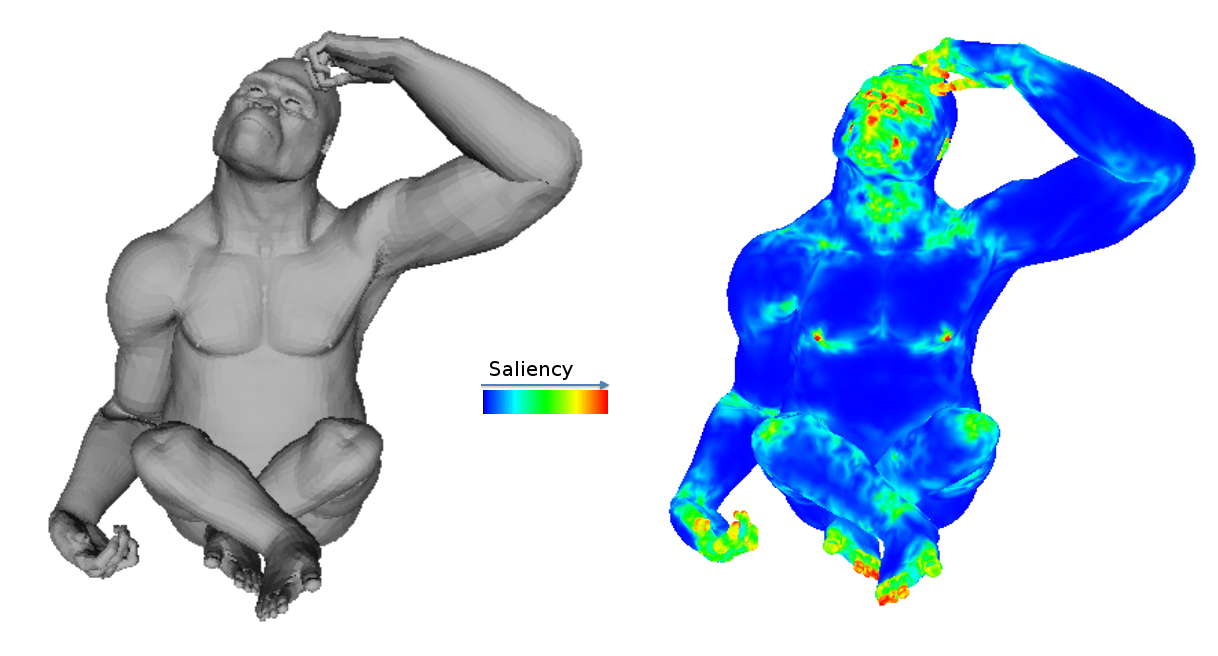
\includegraphics[width=1.0\textwidth]{mss_gorilla_alpha.png}\\ % PNG-File
  \caption{A multi-scale mesh saliency map for an object including color scale. Published by Nouri \textit{et al.} \cite{nouri2015multi}}\label{fig:gorilla_saliency_map}
\end{figure}

Consider figure \ref{gorilla_saliency_map}. It depicts an object and its multi-scale mesh saliency map as well as a scale for reference. The scale describes how yellow and red colored vertices indicate high mesh saliency values for those vertices while green and blue colored ones suggest lower values. Note that this map is not computed via the \textit{standard} mesh saliency model but an enhanced, multi-scale based one. The figure is suitable to explain the idea behind which point-wise difference value in user and mesh saliency values are \textit{weighted} in this work.

Based on the assumption that a difference betwen \textit{mesh} and \textit{user saliency} values of a vertex is more interesting if it is surrounded by vertices which have high \textit{mesh saliency} values than it would be if all the surrounding vertices are deemed not highly interesting by \textit{mesh saliency}, such differences get weighted. Consider a vertex $v_i$ in the following cases.

\begin{description}
	\item [case 1:] $v_i$ has a \textit{user saliency} value of 0.2 or lower and vertices in $V_{proximty}(v_i)$ have an average \textit{mesh saliency} value of $\omega$ or higher.
	\item [case 2:] $v_i$ has a \textit{user saliency} value of 0.2 or lower and vertices in $V_{proximty}(v_i)$ have an average \textit{mesh saliency} lower than $\omega$
	\item [case 3:] $v_i$ has a \textit{user saliency} value of 0.8 or higher and vertices in $V_{proximty}(v_i)$ have an average \textit{mesh saliency} value of $\omega$ or higher
	\item [case 4:] $v_i$ has a \textit{user saliency} value of 0.8 or lower and vertices in $V_{proximty}(v_i)$ have an average \textit{mesh saliency} lower than $\omega$
\end{description}

This simple evaluation process is based on the assumption that realistic, reliable results are achieved by the model of \textit{mesh saliency}. So it focuses on finding deviations within parts and regions of objects that have high average mesh saliency values. Thus, only in cases 1 and 3, vertex-wise differences get weighted. High vertex-wise differences in regions with a low overall mesh saliency value still are considered for the final \textit{weighted difference ratio}, but not as much as those at hand in cases 1 and 3.

Regarding how the actual weighting is done, a simple function that increases the vertex-wise \textit{raw difference} values, normalising them between 0.0 and 1.0 without getting greater than 1.0 is used. An altered, restricted function describing a circle that has its centre at $x = 1.0, y = 0.0$ and radius $r = 1.0$ is suitable for this demand. Figure \ref{fig:weighting_function} depicts this \textit{weighting function}. It shows how vertex-wise differences between \textit{mesh saliency} and \textit{user saliency} values are used for computation of the final, overall difference ratios - both \textit{unweighted} (black line) and \textit{weighted} (blue curve).

\begin{figure}[htb]
  \centering
  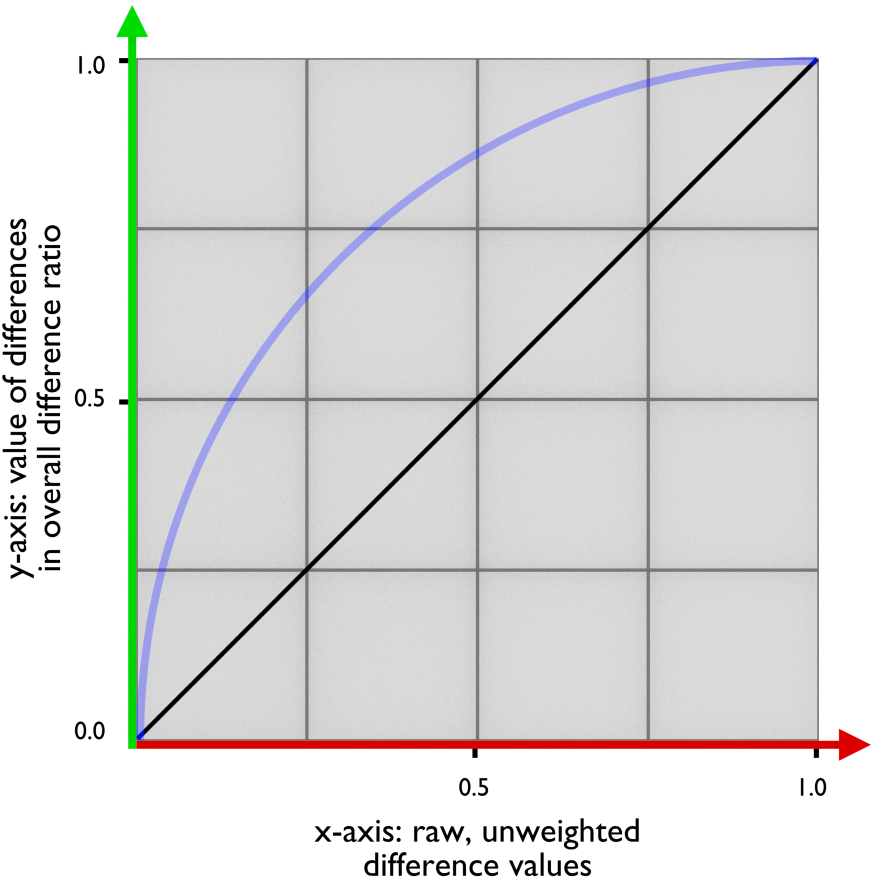
\includegraphics[width=.7\textwidth]{weighting_function.png}\\ % PNG-File
  \caption{Graphic representation of the weighting function in relation to the \textit{unweighted} difference values (straight, black line)}\label{fig:weighting_function}
\end{figure}

Consider figure \ref{fig:weighting_function}. The straight, black line, being a steady identity function of float values, shows normalised \textit{unweighted} vertex-wise difference values. For such values, both in regards to \textit{unweighted} and \textit{weighted} overall \textit{difference ratios}, their unaltered, absolute value $\Delta_{raw}(v_i)$ is used for computation. However, should vertices in $V_{proximty}(v_i)$ have an average \textit{mesh saliency} value of $\omega$ or greater, the difference between \textit{mesh saliency} and \textit{user saliency} values at $v_i$ is weighted according to the blue curve function shown in the figure.

In conclusion, if $v_i$ is surrounded by vertices whose average of computed \textit{mesh saliency} values surpasses a certain threshold $\omega$, it is assumed that $v_i$ is located in a greater, contiguous patch of the object with high importance as determined by the processing according to \textit{mesh saliency}. Hence, $\Delta_{raw}(v_i)$ is used for generating the overall \textit{unweighted difference ratio} and $\Delta_{weighted}(v_i)$ is used used for generating the overall \textit{weighted difference ratio}.

		\subsection{step-wise summery}
		\label{sec:ste_wise_summery}
This subsection provides a brief summary of the steps to computing overall \textit{unweighted} and \textit{weighted difference ratios} described in greater detail in the precedig subsections. It provides more insight into how the data is organised and prepared for evaluation. It describes the workflow for a single 3D object.

\begin{enumerate}
	\item Compute the \textit{mesh saliency} map for a given object using using \texttt{climberpi's} implementation \cite{clms} and store the result in an external textfile \texttt{computed\_saliency} for later use.
	\item Read \textit{n} textfiles \texttt{u\_00}, ... \texttt{u\_n}, each containing one user selection, compute the \textit{user saliency} map based on how many times each vertex was selected in relation to the most-selected vertices and store the result in an external textfile \texttt{user\_saliency} for later use.
	\item Read \texttt{computed\_saliency} and \texttt{user\_saliency}, store the contents in two containers of type \texttt{std::vector} called \textit{computed\_saliency\_values} and \textit{user\_saliency\_values}.
	\item calculate vertex-wise saliency differences and store them in an a \texttt{std::vector} \textit{differences\_unweighted}.
	\item Iterate through the list of vertices of the currently considered object. For every such vertex $v_i$, find vertices $v_1$, ... $v_j$ $\in$ $V_{proximty}(v_i)$ via a range-query to the \texttt{ocTree} instance indexing the object (see section \ref{sec:addVerticesToSelectionByCoordinates()}).
	\item For each vertex $v_i$, look up \textit{mesh saliency} values for vertices $v_1$, ... $v_j$ in the \textit{mesh saliency} map. Compute the average of those values.
	\begin{enumerate}
		\item if average is $\omega$ or greater, compute $\Delta_{weighted}(v_i)$ and storte it in a \texttt{std::vector differences\_weighted}.
		\item if average is less than $\omega$, keep $\Delta_{raw}(v_i)$ as it is in \texttt{differences\_unweighted}.
	\end{enumerate}
	\item Iterate through \texttt{differences\_unweighted}, calculate the average and return it as the overall \textit{unweighted difference ratio}.
	\item Iterate through \texttt{differences\_weighted}, calculate the average and return it as the overall \textit{weighted difference ratio}
\end{enumerate}

